\documentclass[11pt,fleqn]{article}
\usepackage[margin=1in,top=1in,bottom=1in]{geometry}
\usepackage{tikz}
\usepackage{mathtools}
\usepackage{longtable}
\usepackage{enumitem}
\usepackage{hyperref}
%\usepackage[dvips]{graphics}
%\usepackage[table]{xcolor}
%\usepackage{amssymb}
\usepackage{float}
%\usepackage{subfig}
\usepackage{booktabs}
\usepackage{subcaption}

\usepackage[normalem]{ulem}

\usepackage{multicol}
\usepackage{txfonts}
\usepackage{amsfonts}
\usepackage{natbib}
\usepackage{gb4e}
\usepackage[all]{xy}
\usepackage{rotating}
\usepackage{tipa}
\usepackage{multirow}
\usepackage{authblk}
\usepackage{url}
\usepackage{pdflscape}
\usepackage{rotating}
\usepackage{adjustbox}
\usepackage{array}


\def\bad{{\leavevmode\llap{*}}}
\def\marginal{{\leavevmode\llap{''}}}
\def\verymarginal{{\leavevmode\llap{''''}}}
\def\swmarginal{{\leavevmode\llap{4}}}
\def\infelic{{\leavevmode\llap{\#}}}

\definecolor{airforceblue}{rgb}{0.36, 0.54, 0.66}
%\definecolor{gray}{rgb}{0.36, 0.54, 0.66}

\definecolor{Pink}{RGB}{240,0,120}
\newcommand{\red}[1]{\textcolor{Pink}{#1}}
\newcommand{\jd}[1]{\textbf{\textcolor{Pink}{[jd: #1]}}}

\newcommand{\dashrule}[1][black]{%
  \color{#1}\rule[\dimexpr.5ex-.2pt]{4pt}{.4pt}\xleaders\hbox{\rule{4pt}{0pt}\rule[\dimexpr.5ex-.2pt]{4pt}{.4pt}}\hfill\kern0pt%
}

\setlength{\parindent}{.3in}
\setlength{\parskip}{0ex}

\newcommand{\yi}{\'{\symbol{16}}}
\newcommand{\nasi}{\~{\symbol{16}}}
\newcommand{\hina}{h\nasi na}
\newcommand{\ina}{\nasi na}

\newcommand{\foc}{$_{\mbox{\small F}}$}

\hyphenation{par-ti-ci-pa-tion}

\setlength{\bibhang}{0.5in}
\setlength{\bibsep}{0mm}
\bibpunct[:]{(}{)}{,}{a}{}{,}

\newcommand{\6}{\mbox{$[\hspace*{-.6mm}[$}} 
\newcommand{\9}{\mbox{$]\hspace*{-.6mm}]$}}
\newcommand{\sem}[2]{\6#1\9$^{#2}$}
\renewcommand{\ni}{\~{\i}}

\newcommand{\citepos}[1]{\citeauthor{#1}'s \citeyear{#1}}
\newcommand{\citeposs}[1]{\citeauthor{#1}'s}
\newcommand{\citetpos}[1]{\citeauthor{#1}'s (\citeyear{#1})}

\newcolumntype{R}[2]{%
    >{\adjustbox{angle=#1,lap=\width-(#2)}\bgroup}%
    l%
    <{\egroup}%
}
\newcommand*\rot{\multicolumn{1}{R{90}{0em}}}% no optional argument here, please!


\title{Exp 13 write-up}

\author{Judith Tonhauser}

\newcommand{\jt}[1]{\textbf{\color{blue}JT: #1}}

\begin{document}

\maketitle

\vspace*{-1cm}

\section{Introduction}\label{s-intro}

On the basis of observed gradient mean certainty ratings for the contents of the complements (CCs) of 20 clause-embedding predicates, \citealt{degen-tonhauser-openmind,degen-tonhauser-language} suggested:

\begin{itemize}
\item[a)] projection is gradient, that is, it is not the case that content either projects or it doesn't, but rather content projects to varying degrees, reflecting varying degrees of (of certainty of the interpreter about) speaker commitment, and

\item[b)] that there is no empirical support (to date) for a binary division between factive and non-factive predicates, that is, between predicates that conventionally code that the CC is presupposed and predicates that do not code such a requirement.
\end{itemize}

 \citealt[\S6.2]{mandelkern-etal2020} argued that the observed gradience is due to the inference task used. They suggested that acceptability ratings in explicit ignorance contexts are better suited to investigating projection and, specifically, to distinguishing presuppositions (conventionally specified projective content) from other projection inferences: ``we should think twice before embracing a notion of presupposition projection that is gradient based on results from inference tasks alone'' (p.497). 

More specifically, \citealt{mandelkern-etal2020} argued that just because participants ``tend to draw certain inferences from clauses appearing in embedded, entailment-canceling environments, does not necessarily mean that the relevant content has projected in the sense that theorists of presupposition should care about'' (p.497). They suggest that it ``may well be that inference tasks to some degree invite subjects to make the inference in question if it is compatible with the assertion, since the content in question is right there before the subjects' eyes'' (p.498). They argued that acceptability ratings of sentences presented in explicit ignorance contexts are better suited to distinguish conventionally specified projective content from other projection inferences: if participants ``draw an inference just because it is a natural conclusion to draw for any of a variety of pragmatic reasons short of entailment or presupposition, then they will tend to relinquish that inclination when there is pragmatic pressure to do so [...]. By contrast, if the inference in question is a semantic presupposition, this will not be a possibility: beyond the (marked) rescue mechanism of local accommodation, subjects will not have an alternative to interpreting the presupposition at the utterance level, and in turn seeing the utterance as infelicitous and the speaker as incoherent'' (p.497).

p.497: ``In methodological terms, we strongly recommend at least a two-pronged approach, with careful attention paid to results stemming from the evaluation of acceptabilty [sic] in different contexts.''

We conducted an experiment that was designed to investigate \citepos{mandelkern-etal2020} claim that gradient projection is due inference ratings and will not be observed acceptability ratings in explicit ignorance contexts. We hypothesize that acceptability ratings in explicit ignorance contexts will also yield gradient distinctions between the CCs of the 20 clause-embedding predicates investigated in \citealt{degen-tonhauser-openmind,degen-tonhauser-language}, rather than revealing a binary distinction between factive and non-factive predicates.\footnote{Preregistration of our experiment: \url{https://osf.io/5fsku}}

\section{\citealt{mandelkern-etal2020}}

\begin{itemize}

\item This paper is concerned with the question of whether ``the mechanism behind presupposition projection and filtering [is] fundamentally asymmetric or symmetric'' (p.473). To this end, they investigated presupposition filtering in conjunctions, and whether there is evidence for both left-to-right filtering and right-to-left filtering, or only the former.

\item Assumptions

\begin{itemize}

\item Local accommodation is ``marked'' (p.497).

\begin{exe}
\ex  I don't know if Sue has ever played piano. Did Sue play the piano again?
\\ Global accommodation (default): unacceptable
\\ Local accommodation (marked): Did Sue played the piano and did she play it again?
\end{exe}

\item p.478: ``Local accommodation in general encompasses cases in which presuppositions triggered in entailment-canceling environments that generally project presuppositions, like negation and antecedents of conditionals, do not wind up as inferences supported by the utterance as a whole. In assessing the filtering properties of complex sentences, it is thus crucial to distinguish failure to project due to local accommodation from failure to project due to filtering, either left-to-right or right-to-left. As we discuss below, our experimental designs accomplish this by including a simple presuppositional control condition where failure to project can only be due to local accommodation, thus providing a baseline relative to which any separate effects of filtering can be assessed.''

\item p.480:

\begin{exe}
\exi{(11)} Simple Ps:\\
If Mary stopped doing yoga, then Matthew will interview her for his story.
\end{exe}

Controls like (11) provide a baseline for projection. The only thing that could prevent projection from a sentence like (11) would be local accommodation. Therefore rates of projection out of sentences like this one will provide a baseline for projection in the task. To the extent that the critical variants with conjunctive antecedents exhibit the use of an additional mechanism to prevent projection, namely filtering, this should be reflected in relatively lower inference endorsement rates than in the simple control variants, where the only mechanism that could prevent projection is local accommodation.''


\end{itemize}

\item Materials Exp.~3

\begin{itemize}

\item Two contexts

\begin{exe}
\ex 
\begin{xlist}
\ex Support context: Jacob has been traveling a lot, and he's in France this week.
\begin{xlist}
\ex If Emily is \underline{happy} that Jacob is in France, then she will call him soon. \hfill (simple ps, not a critical condition)
\ex If Emily is \underline{happy} that Jacob is in France and he is in Paris, then she will call him soon. \hfill (ps in first conjunct)
\ex If Jacob is in Paris and Emily is \underline{happy} that he is in France, then she will call him soon. \hfill (ps in second conjunct)
\end{xlist}

\ex Explicit ignorance context: Jacob has been traveling a lot, but I'm not sure where he is this week.

\end{xlist}
\end{exe}

\item 4 ps triggers: {\em is happy, is aware, has stopped, continues V{\em ing}} (six lexicalizations each)
\\ 4 non-ps triggers: {\em was hoping, is sure, now frowns on, enjoys V{\em ing}} (same six lexicalizations as the ps variant)\footnote{It is not clear that {\em X now frowns on Ving} doesn't presuppose that X Ved in the past. 
\begin{exe}
\exi{(i)} Emily used to enjoy boardgames, \{and she also loved playing with toys when she was little / but I don't know whether she ever played with toys\}. If Emily \{has stopped / now frowns on\} playing with toys and she used to play with toy cars, then Jacob will buy her racing video games for her birthday.
\end{exe}
}

\item ``24 critical items in a total of 12 versions''
\\ 4 ps triggers x 6 lexicalizations = 24 critical items
\\ 12 versions = 3 (no conjunct vs first vs second conjunct) x 2 (ps vs no ps) x 2 contexts 

The factors ``ps vs no ps'' and ``context'' were between subject.

p.491: ``Second, precluding participants from seeing both presuppositional and non-presuppositional variants aimed to avoid any potential confusion or noise due to lack of attention to the particular verb seen in a given trial; it also aimed to prevent strategic effects and insights into the manipulation from arising. Similar concerns arose for the context manipulation, though note that through the fillers, detailed below, each participant did see some variety of contexts throughout the entire experiment.''

p.492: ``all participants saw at least 16 equivalents of Support contexts, and 16 equivalents of Expl-Ign contexts, regardless off which type of context their group was assigned to for the critical items.''


\end{itemize}

\item Procedure: ``How natural is the sentence in the given context?", ratings given in 7-point Likert scale, with points labeled `completely unnatural' and `completely natural'

\item Participants: 126 students (no mention of exclusion criteria)

\item Analysis (linear mixed effects model): Compare naturalness ratings of ps triggers and non-ps triggers in explicit ignorance context to naturalness ratings in support context.

``Thus comparing contexts which support the inference to contexts in which it has been made clear that the speaker is ignorant about the inference provides a way to distinguish a broad class of natural and invited pragmatic inferences from those that are really encoded as presuppositions, and thus {\bf have no choice but to project}.'' (p.497, bold-face added).

\item Results

\begin{itemize}

\item p.492: ``the Simple-Ps condition exhibits low ratings for the Expl-Ign context, but high ratings for the Support context, establishing the effectiveness of the methodology. Next, the non-presuppositional conjunctive conditions, [...] also do not seem to exhibit any variation by context or, for that matter, conjunct order. Turning to the critical conditions, the conditions with the trigger in the second conjunct also seem comparably acceptable across contexts. Only when the trigger is introduced in the first conjunct does context seem to matter, with lower ratings in the Expl-Ign context.''

\item p.494: ``As a further point, it's worth highlighting that the overall pattern is remarkably uniform across triggers (see graph showing results by trigger in Appendix for details). While the acceptability of both Simple-Ps and Ps-First varies across triggers (with particularly high acceptability for {\em aware}, perhaps due to relative ease of local accommodation for this trigger), the two conditions show comparable acceptability levels in Expl-Ign for each of the triggers.''

\end{itemize}

\end{itemize}

\section{This experiment, and expectations}

\begin{itemize}

\item In this experiment, we will investigate the projection of the CCs of the 20 clause-embedding predicates using an acceptability rating task that is similar to that of \citealt{mandelkern-etal2020}. 

\item Like MEAL, we place our target stimuli (400 interrogatives from \citealt{degen-tonhauser-openmind, degen-tonhauser-language}) in an explicit ignorance context, where the speaker is explicitly not committed to the CC. 

\begin{exe}
\ex
\begin{xlist}
\ex I have no idea if Julian dances salsa. Did Cole discover/say that Julian dances salsa?
\ex Julian is German. Did Cole discover/say that Julian dances salsa?
\ex Julian is Cuban. Did Cole discover/say that Julian dances salsa?
\end{xlist}
\end{exe}

\item Instead of MEAL's `support' context (which entails the CC), we use `neutral' contexts, which are compatible with the CC but don't entail it. (\citealt{brst-lang11} called such contexts neutral, contrasting them with positive, which is like their support context.) These `neutral' contexts are given by the low and high prior probability facts of \citealt{degen-tonhauser-openmind}: Regardless of whether Julian is German (low prior probability fact) or Cuban (high prior probability fact), he may or may not dance salsa.

Using these two types of `neutral' context allows us to identify whether acceptability ratings are also sensitive to the content's prior probability. It also gives us a comparison between contexts where the speaker is explicitly ignorant about the CC vs not explicitly ignorant but possibly ignorant.

\item Predictions presupposition analysis:

\begin{exe}
\ex Explicit ignorance context:
\begin{xlist}
\ex Presupposition triggers: acceptable only under local accommodation, which is marked
\ex Non-ps triggers: acceptable because no ps is triggered
\end{xlist}
\ex Neutral context
\begin{xlist}
\ex Ps triggers: acceptable, since global accommodation is possible, and ``default'' and ``unmarked'', no sensitivity to prior probability predicted
\ex Non-ps triggers: acceptable, since no ps is triggered, but inference comes about pragmatically, sensitivity to prior probability expected
\end{xlist}
\end{exe}

\item Given \citealt{degen-tonhauser-openmind}, we expect that acceptability ratings are also sensitive to these prior probabilities. If so, researchers who want to maintain the difference between factive and non-factive predicates will have to assume that accommodation is sensitive (for factives) and whatever the mechanism for projection is for non-factives is also sensitive.

\item \citealt{mandelkern-etal2020} lead us to expect a binary distinction in acceptability ratings in explicit ignorance contexts between expressions that conventionally code presuppositions and expressions whose content projects for pragmatic reasons: The former are expected to have lower ratings than the latter.

\item \citealt{mandelkern-etal2020} also lead us to expect a binary distinction in the effect of context on acceptability ratings between expressions that conventionally code presuppositions and expressions whose content projects for pragmatic reasons: For the former, a difference is expected, but not for the latter, or, at least, the difference is expected to be greater for the former than for the latter. 

\item Given \citealt{degen-tonhauser-openmind,degen-tonhauser-language}, we expect acceptability ratings in an explicit ignorance context to  reveal gradient projection. 

\item Given \citealt{brst-lang11}, we expect SCF+ expressions, namely {\em too} and {\em also}, to be maximally unacceptable in such contexts.

\item \citealt{abusch10} leads us to expect that it-clefts receive low acceptability ratings since it is a hard trigger, like {\em too}.

\item However, even if we find evidence for gradient projection from acceptability ratings in an explicit ignorance contexts, researchers like \citealt{mandelkern-etal2020} can always use variation in the ``ease of local accommodation'' (p.494) to account for projection variation. 

\end{itemize}


\section{Methods}\label{s-methods}

\subsection{Participants}

We recruited 425 participants on Prolific. Due to a server error, the data of only 398 participants was recorded (ages: 19-73, median: 40.8; 187 women, 201 men, 8 non-binary, 2 preferred to not disclose). The recruited participants were required to live in the USA, to speak English as their first language, to have completed at least 100 tasks, and to have an approval rating of at least 99\%. The median time spent on the task was 6:24 minutes. Participants were paid \$1.78 (corresponding to an hourly pay of \$16.6).


\subsection{Materials}

The materials consisted of two-sentence discourses that were uttered by a named speaker: As shown in the sample target stimuli in (\ref{sample}), the first sentence was always a declarative sentence and the second one an interrogative sentence. 

\begin{exe}
\ex\label{sample}
\begin{xlist}
\ex I have no idea if Julian dances salsa. Did Cole discover that Julian dances salsa?
\ex Julian is German. Did Cole discover that Julian dances salsa?
\ex Julian is Cuban. Did Cole discover that Julian dances salsa?
\end{xlist}
\end{exe}

In the target stimuli, the interrogative sentences were identical to those of \citealt{degen-tonhauser-openmind,degen-tonhauser-language}: they were constructed from 20 clause-embedding predicates paired with 20 clauses, as shown in (\ref{sample}) for the predicate {\em discover} and the clause {\em Julian dances salsa}. There were two context conditions: In the `explicit ignorance' context, illustrated in (\ref{sample}a), the declarative sentence that preceded the interrogative conveyed that the speaker is ignorant about the content of the embedded clause. In the `neutral' context, illustrated in (\ref{sample}b-c), the declarative sentence conveyed a fact about the subject of the embedded clause that is compatible with the projection of the CC. These facts are identical to the low and high prior probability facts of \citealt{degen-tonhauser-openmind}.  


The experiment also included 6 filler stimuli, which were only presented in an explicit ignorance context and were the same for each participant. They include ``again'' (prejacent), ``stop'' (pre-state content), ``continue'' (pre-state content), for comparison with \citealt{mandelkern-etal2020} and \citealt{kalomoiros-schwarz2021}, as well as ``too'' (prejacent), ``also'' (prejacent) and an it-cleft (existential closure over relative clause), because \citealt{abusch10} proposed that these are hard triggers. (Prosody was not controlled: the assumption is that the  presuppositions of {\em too, also} and the it-cleft cannot be accommodated so these triggers, if indeed hard, should receive low acceptability ratings under any focus assignment.)

\begin{exe}
\ex Filler stimuli
\begin{xlist}
\ex I don't know if Ann plays any instrument. Does Ann play the flute, too?
\ex I don't know if Svenja plays any sport. Does Svenja also play soccer?
\ex I don't know if anyone was playing outside with the kids. Was it Jack who was playing outside with the kids?
\ex I don't know if Stephen was ever in the habit of vaping. Has Stephen recently stopped vaping?
\ex I don't know if John was ever reading ``Dune''. Has John recently continued reading ``Dune''?
\ex I don't know if William was ever interested in history. Is William interested in history again?"
\end{xlist}
\end{exe}

Finally, the experiment included 4 control stimuli, which were used to exclude participants not attending to the task. These were expected to be rated as natural/acceptable.

Each participant saw a random set of 30 stimuli: Each set contained one target utterance for each of the 20 CCs (each paired with a unique clause-embedding predicates), the same 6 control stimuli, and the same 4  filler stimuli. 12 of the CCs were presented in the explicit ignorance context, 4 with a low prior probability fact, 4 with a high prior probability fact. Within-block trial order was randomized. After completing the experiment, participants filled out a short optional demographic survey. To encourage truthful responses, participants were told that they would be paid no matter what answers they gave in the survey.

The experiment started off with four practice trials (2 natural, 2 unnatural; participants were given feedback on correct and incorrect answers).


\subsection{Data exclusion} 

We excluded the data of five participants who did not self-declare to be native speakers of American English. We also excluded the data of 23 participants whose mean response to the controls was more than 2 sd below the group mean.\footnote{Only three of the four controls were used to exclude participants. While three of the four controls received high acceptability ratings, as expected (mean: .86), the fourth control, shown in (i), only received a mean rating of 0.5. 
\begin{exe}
\exi{(i)} Hendrick was looking to buy a car. Was Hendrick's car expensive?
\end{exe}
} The data of 370 participants entered into the analysis (ages: 19-80, mean: 40.7; 175 women, 185 male, 8 non-binary, 2 preferred to not disclose). 

\section{Results}

Data points:

\begin{itemize}

\item Each predicate and each CC received 370 ratings. 

\item Each of the 60 predicate/context combinations received at least 59 ratings (median: 80, mean: 123).

\item Each predicate received at least 200 ratings in the explicit ignorance context (median: 224.5, mean: 222).

\item Each predicate received at least 59 ratings in each of the neutral contexts (median: 75, mean: 74).

\end{itemize}
 
\subsection{Is projection binary or gradient?}

Is projection binary, as suggested in \citealt{mandelkern-etal2020}, or gradient, as suggested in \citealt{degen-tonhauser-openmind,degen-tonhauser-language}?

\begin{figure}[h!]
\centering
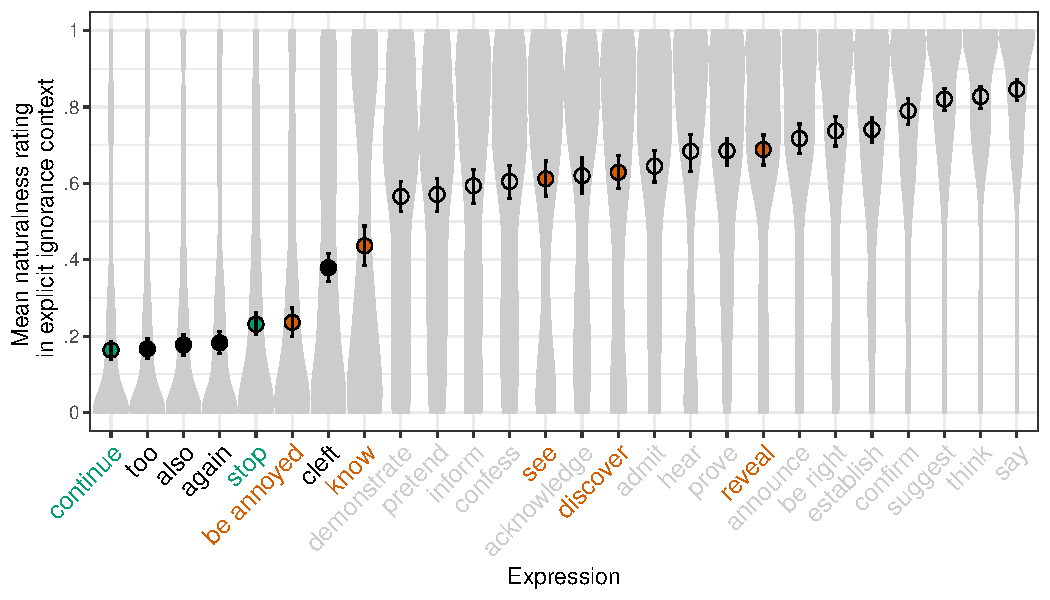
\includegraphics[width=\textwidth]{../../results/main/13explicitIgnorance/graphs/explicit-ignorance-naturalness-by-predicate}
\caption{Mean naturalness ratings in explicit ignorance contexts by expression. Error bars indicate 95\% bootstrapped confidence intervals. Violin plots indicate the kernel probability density of the individual participants' ratings. Fillers are given in gray, factive predicates in red.}\label{fig:acc-by-expression}
\end{figure}

\begin{itemize}

\item \citealt{brst-lang11} classified the prejacent of {\em too} and {\em also} as +SCF content, that is, content that cannot be (globally or locally) accommodated. As expected, these expression/content pairs receive among the lowest acceptability ratings in explicit ignorance contexts.

\item \citealt{brst-lang11} classified the pre-state contents of {\em stop} and {\em continue} as -SCF content, that is, content that can be accommodated. \citealt{tbd-variability} observed that the pre-state content of {\em stop} is projective, but not at ceiling. Against this background, the very low mean acceptability ratings, especially for {\em continue}, are unexpected. They suggest that the pre-state contents resist local accommodation (if ps is triggered) or are strongly projective.

\item \citealt{abusch10} assumed that {\em it-}clefts are hard triggers, that is, unacceptable in explicit ignorance contexts. Our results are more in line with the results of \citealt{smith-hall-cls}, who also did not observe strong projection for the cleft.

\item Contrary to what \citealt{mandelkern-etal2020} suggested, there is no binary distinction between factive and non-factive predicates: The mean acceptability ratings for several factive predicates ({\em see, discover, reveal}) are at least as high as that of non-factive predicates.  The mean acceptability rating of {\em know} is not at floor (notice the bimodal responses!). The mean rating of {\em be annoyed} is higher than that of {\em too} and {\em also}.

\end{itemize}

\subsection{Difference between naturalness ratings in explicit ignorance and neutral contexts?}

\citealt{mandelkern-etal2020} did not merely compare acceptability ratings of presuppositions and non-presuppositions in explicit ignorance contexts, but they rather claimed that there is a difference in the acceptability ratings in the two contexts between presuppositions and non-presuppositions. Specifically, while there is no difference for non-presuppositions, the ratings for presuppositions are lower in the explicit ignorance context than in the support context.

For comparison with their way of presenting the results, Fig.~\ref{fig:acc-by-context2} plots the mean acceptability ratings by expression and context (distinguishing explicit ignorance from neutral), with the expressions sorted by the difference between the mean rating in the two contexts: The mean rating in the neutral context is higher than the mean rating in the explicit ignorance context for {\em be annoyed}; the opposite is the case for {\em confirm}.

\begin{figure}[h!]
\centering
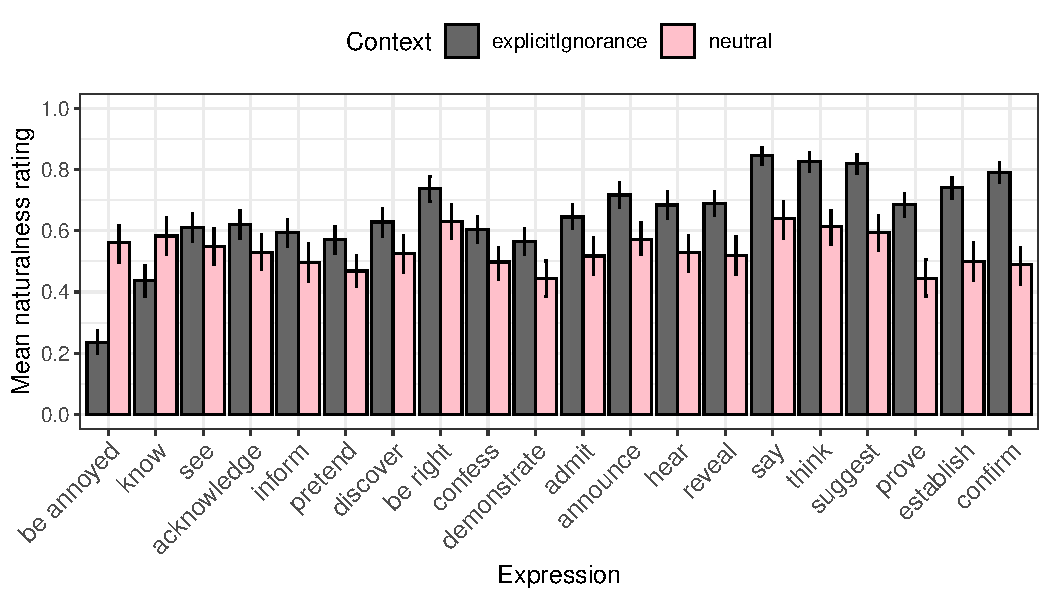
\includegraphics[width=\textwidth]{../../results/main/13explicitIgnorance/graphs/naturalness-by-context2-and-predicate}
\caption{Mean naturalness ratings by expression and context. Error bars indicate 95\% bootstrapped confidence intervals.}\label{fig:acc-by-context2}
\end{figure}

\begin{itemize}

\item For {\em be annoyed} and {\em know}, the mean rating in the explicit ignorance context is lower than the mean rating in the neutral context, suggesting that the interrogatives are judged to be less neutral when the speaker is explicitly ignorant about the truth of the CC. 

For {\em see}, the mean rating in the two contexts does not appear to be different (but model suggests neutral is already higher), and the pattern seems to go in the opposite direction for {\em discover} and {\em reveal}. 

Thus, on this way of displaying the data, too, factive predicates do not show a homogenous pattern that distinguishes them from non-factive predicates.

\item Non-factive predicates also do not show a homogenous pattern: For some predicates, the ratings in the two contexts do not appear to be different (e.g., {\em acknowledge, inform}), while ratings in the explicit ignorance context seem to be higher than in the neutral context for other predicates (e.g., {\em say, confirm}).

\item When ratings are higher in explicit ignorance than neutral contexts, this suggests that a natural use of these predicates is for the speaker to inquire about the CC, given their explicit ignorance.

\end{itemize}

\subsection{The effect of the prior probability of the CC on naturalness ratings}

Fig.~\ref{fig:acc-by-context} plots the mean acceptability ratings by expression and context (distinguishing explicit ignorance from factL and factH), with the expressions sorted on the mean acceptability rating in the explicit ignorance context, as in Fig.~\ref{fig:acc-by-expression}.

\begin{figure}[h!]
\centering
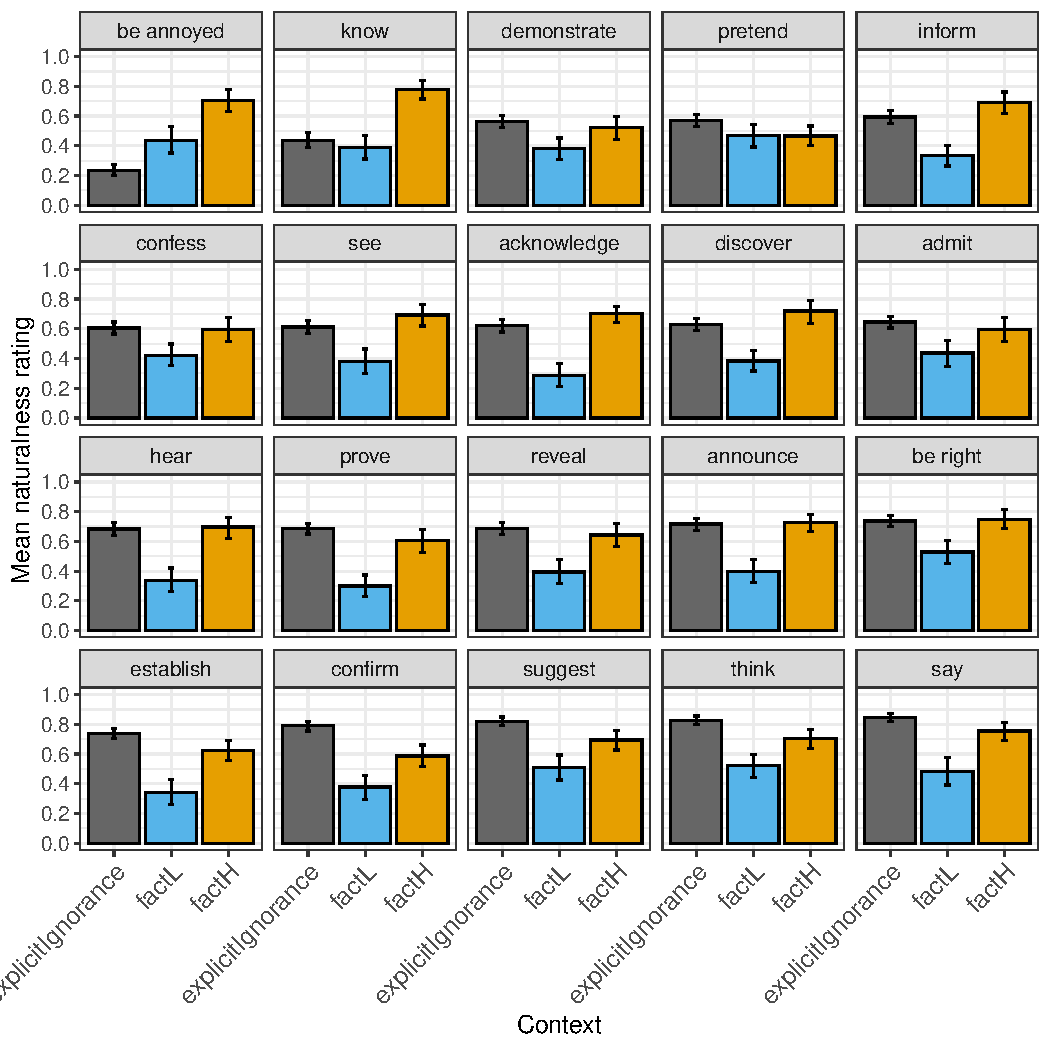
\includegraphics[width=.8\textwidth]{../../results/main/13explicitIgnorance/graphs/naturalness-by-context-and-predicate}
\caption{Mean naturalness ratings by expression and context. Error bars indicate 95\% bootstrapped confidence intervals.}\label{fig:acc-by-context}
\end{figure}

\begin{itemize}

\item For all predicates except {\em pretend} (and {\em admit}?), the acceptability ratings are higher in factH contexts than in factL contexts. This observation suggests that acceptability ratings are sensitive to the prior probability of the CC. This is true regardless of whether ratings in explicit ignorance contexts are higher or lower or similar to those in neutral contexts.

This observation suggests that it is generally more acceptable for a speaker to ask about some AH's relation to the CC in a context in which the speaker assigns a higher probability to the CC than in a context where the speaker assigns a lower probability to the CC.

\item {\em be annoyed} and {\em know} show distinct patterns: For {\em be annoyed}, ratings are higher in the factH context than in the factL context, and higher in the factL context than in the explicit ignorance context. For {\em know}, the latter two ratings do not differ. So even these two predicates don't show the same pattern in this task. 

\begin{itemize}

\item Assuming that both predicates are factive and trigger a ps doesn't capture why they show these different patterns.

\item {\em be annoyed:} According to \citealt{karttunen2016}, this predicate codes that the AH believes the CC. Belief of the speaker in the CC arises as long as there is no contextual evidence/information that would justify why the speaker wouldn't share the belief. In the explicit ignorance context, the speaker has gone on record that they are ignorant about the CC, that is, do not share in the AH's belief. Given the assumption that {\em be annoyed} only codes AH belief in the CC, the very low acceptability ratings in explicit ignorance contexts are not accounted for. 

\item An explanation may have to do with at-issueness: The explicit ignorance context makes the question ?CC at-issue, but  the interrogative makes the CC not-at-issue, resulting in lower acceptability ratings. 

\item The same explanation may also work for the fillers with {\em stop} and {\em continue}: The explicit ignorance context makes the pre-state content at-issue, but the interrogative makes it not-at-issue.

\item The CC of {\em know} is still quite not-at-issue, but not as much as that of {\em be annoyed}. {\bf need to check this in our other data}

\end{itemize}

\item For predicates other than {\em be annoyed} and {\em know}, acceptability ratings in explicit ignorance contexts are roughly comparable to those in factH contexts. That is, asking whether an AH has a relation to the CC is just as acceptable in a context in which the speaker is explicitly ignorant of the CC and in a context in which the speaker has a belief relative to which the CC has a high probability.

It is when the speaker has a belief relative to which the CC has a low probability that the acceptability ratings are lowest (except with {\em pretend}).


\end{itemize}

\newpage

Here the predicates are ordered by the mean certainty rating (Language paper, Exp.1a).

\begin{figure}[h!]
\centering
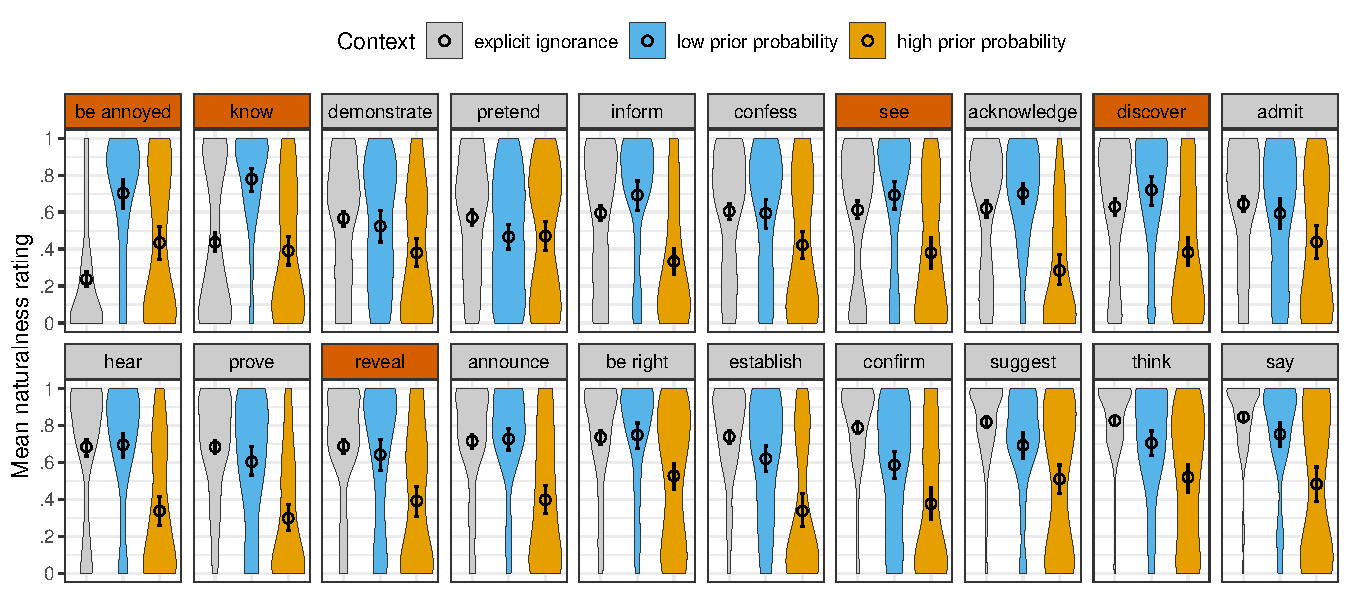
\includegraphics[width=.8\textwidth]{../../results/main/13explicitIgnorance/graphs/ORDER-by-LANGUAGE-naturalness-by-context-and-predicate}
\caption{Mean naturalness ratings by expression and context. Error bars indicate 95\% bootstrapped confidence intervals.}\label{fig:acc-by-context}
\end{figure}


%
%Expectations:
%    - Mandelkern et al 2020: presupposition triggers (factives) have lower naturalness ratings in explicit ignorance context than neutral context than non-factives, for which no difference is expected.
%    - Degen & Tonhauser 2022: the differences between the two contexts are gradient across the 20 predicates, without a clear distinction between factive and non-factive predicates.
%
%Models (fit only to target data):
%
%A. naturalness rating ~ factivity (RL: factive) * context (RL: explIgnorance), by-item (combination of predicate and CC) and by-participant intercepts, factivity slope for participant, and context slopes for item and participant
%
%Expectations based on Mandelkern et al 2020:
%- significant main effect of factivity, positive coefficient: nonfactive predicates better in explIgnorance context than factive ones
%- significant main effect of context, positive coefficient: factive predicates better in neutral context than explIgnorance 
%- interaction: positive coefficient: higher naturalness ratings for nonfactive predicates in neutral context than factive ones in explIgnorance context
%
%?%B. naturalness ~  expression (RL: predicate with smallest naturalness difference between the two contexts) * context (RL: explIgnorance), by-item and by-participant intercepts, and context slopes for item and participant. 
%
%Idea in choosing RL: when there is no difference, this is not a presupposition trigger.
%
%Expectations based on Degen & Tonhauser 2022:
%        - main effect of expression: 
%            - positive coefficient: naturalness ratings for the expression in explIgnorance context is higher than for RL expression (suggests projection of CC is easier to suppress)
%            - negative coefficient: naturalness ratings for the expression in neutral context is lower than for RL expression (suggests projection of CC is harder to suppress)
%        - main effect of context (will ideally be not significant at RL, to interpret interaction)
%        - interaction:
%            - positive coefficient: naturalness rating for the expression in neutral context is higher than for RL expression in explIgnorance context (uninteresting)
%            - negative coefficient: naturalness rating for the expression in neutral context is lower than for RL expression in explIgnorance context (uninteresting)
%
%Comparison of models A and B with AIC to identify whether the factivity-based model A or the predicate-based model B capture more variance in the data (see de Marneffe, Simons & Tonhauser 2019 SuB, Degen & Tonhauser 2022).
%

\subsection{Measuring speaker belief in the CC}

Do the naturalness ratings in explicit ignorance contexts and the inference ratings get at the same underlying theoretical construct, namely speaker belief in the CC?

Spearman rank correlation: -.62


\begin{figure}[h!]
\centering
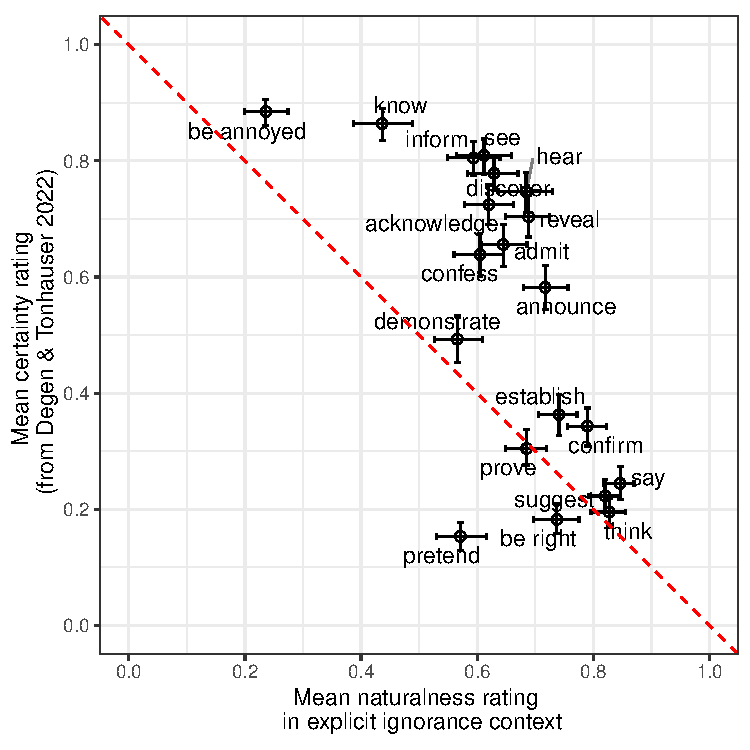
\includegraphics[width=.7\textwidth]{../../results/main/13explicitIgnorance/graphs/mean-acceptability-against-mean-certainty}
\caption{Mean naturalness ratings by mean certainty ratings. Error bars indicate 95\% bootstrapped confidence intervals.}\label{fig:acc-by-certain}
\end{figure}

%
%    - Plot the mean naturalness ratings of the CCs of the 20 clause-embedding predicates against their mean certainty ratings.
%    - Calculate Spearman rank correlation.
%    - If the two measures get at the same underlying theoretical construct, then we expect to find a negative correlation between the two measures such that the higher the mean naturalness rating is (that is, the more the CC does not project), the lower the mean ?certain that? rating.
%
\section{Discussion}\label{s4}

\bibliographystyle{cslipubs-natbib}
\bibliography{/Users/tonhauser.1/Documents/bibliography}

\newpage

\section*{Supplemental materials}

\appendix

\setcounter{page}{1}
%\renewcommand{\thetable}{A\arabic{table}}

\setcounter{table}{0}
\renewcommand{\thetable}{A\arabic{table}}

\setcounter{figure}{0}
\renewcommand{\thefigure}{A\arabic{figure}}

\section{20 clauses}\label{a-clauses}

The contents of the following 20 clauses, which realized the complements of the 20 clause-embedding predicates, were investigated in Exps.~1-3:

\begin{enumerate}[leftmargin=3ex,itemsep=-2pt]

\begin{multicols}{2}

\item Mary is pregnant.
\item Josie went on vacation to France.
\item Emma studied on Saturday morning.
\item Olivia sleeps until noon.
\item Sophia got a tattoo.
\item Mia drank 2 cocktails last night.
\item Isabella ate a steak on Sunday.
\item  Emily bought a car yesterday.
\item  Grace visited her sister.
\item Zoe calculated the tip.

\columnbreak

\item  Danny ate the last cupcake.
\item  Frank got a cat.
\item  Jackson ran 10 miles.
\item  Jayden rented a car.
\item  Tony had a drink last night.
\item  Josh learned to ride a bike yesterday.
\item  Owen shoveled snow last winter.
\item  Julian dances salsa.
\item  Jon walks to work.
\item  Charley speaks Spanish.

\end{multicols}

\end{enumerate}


\section{Participant information and data exclusion criteria}\label{a-participants}

This supplement provides information on the participants of the 12 experiments and the criteria by which participants' data were excluded. The first three columns of Table \ref{t:exclusion} show, for each of the 12 experiments how many participants were recruited, their age range and mean age, and their self-reported gender; no gender data was collected in Exp.~1q. The next three columns provide information on the number of participants whose data were excluded based on the following criteria:

\begin{itemize}[itemsep=-2pt]

\item `multiple': Due to an experimental glitch, some participants participated more than once in Exp.~1q. Since no information was available on which one was their first take, those participants' data was removed. 

\item `language': Participants' data were excluded if they did not self-identify as native speakers of American English.

\item `controls': Participants' data were excluded if their mean rating on the 6 main clause control items in the projection block was more than 2 sd above the group mean (in Exps.~1q, 2q, and 3q) or more than 2 sd below the group mean (in the remaining experiments). Participants' data were also excluded if their mean rating on the 6 main clause control items in the at-issueness block was more than 2 sd above the group mean (across all experiments).
 
\item `variance': Participants' data were excluded if they always selected roughly the same point on the response scale for the target stimuli. To identify such participants, we first identified participants whose mean variance on the target stimuli was more than 2 sd below the group mean variance and then manually inspecting their response patterns. The data of participants who used the full scale was not excluded.  
\end{itemize}

The remaining columns of Table \ref{t:exclusion} provide information on the remaining participants, that is, the participants' data that entered into the analysis. Participants took around 9-11 minutes to complete the various experiments. Participants were paid more in Exps.~1c, 2c, and 3c than the remaining experiments because the target stimuli in those experiments were longer (as they consisted of conditionals). More women than men were recruited in many of the experiments because the experiments were run at a time when Prolific went viral on TikTok, resulting in a large number of young women registering for the service (around July 24, 2021; see \url{https://blog.prolific.co/we-recently-went-viral-on-tiktok-heres-what-we-learned/}, \\ last accessed February 4, 2022).  

 
\end{document}

